\documentclass[12pt,twoside]{article}

\newcommand{\reporttitle}{493 Data Analysis and Probabilistic Inference}
\newcommand{\reportauthor}{}
\newcommand{\reporttype}{Notes}
\newcommand{\cid}{}

% include files that load packages and define macros
%%%%%%%%%%%%%%%%%%%%%%%%%%%%%%%%%%%%%%%%%
% University Assignment Title Page 
% LaTeX Template
% Version 1.0 (27/12/12)
%
% This template has been downloaded from:
% http://www.LaTeXTemplates.com
%
% Original author:
% WikiBooks (http://en.wikibooks.org/wiki/LaTeX/Title_Creation)
%
% License:
% CC BY-NC-SA 3.0 (http://creativecommons.org/licenses/by-nc-sa/3.0/)
% 
% Instructions for using this template:
% This title page is capable of being compiled as is. This is not useful for 
% including it in another document. To do this, you have two options: 
%
% 1) Copy/paste everything between \begin{document} and \end{document} 
% starting at \begin{titlepage} and paste this into another LaTeX file where you 
% want your title page.
% OR
% 2) Remove everything outside the \begin{titlepage} and \end{titlepage} and 
% move this file to the same directory as the LaTeX file you wish to add it to. 
% Then add \input{./title_page_1.tex} to your LaTeX file where you want your
% title page.
%
%----------------------------------------------------------------------------------------
%	PACKAGES AND OTHER DOCUMENT CONFIGURATIONS
%----------------------------------------------------------------------------------------
\usepackage{ifxetex}
\usepackage{textpos}
\usepackage{natbib}
%\usepackage{breqn}
\usepackage{kpfonts}
\usepackage[a4paper,hmargin=2.8cm,vmargin=2.0cm,includeheadfoot]{geometry}
\usepackage{ifxetex}
\usepackage{stackengine}
\usepackage{tabularx,longtable,multirow,subfigure,caption}%hangcaption
\usepackage{fncylab} %formatting of labels
\usepackage{fancyhdr}
\usepackage{color}
\usepackage[tight,ugly]{units}
\usepackage{url}
\usepackage{float}
\usepackage[english]{babel}
\usepackage{amsmath}
\usepackage{graphicx}
\usepackage[colorinlistoftodos]{todonotes}
\usepackage{dsfont}
\usepackage{epstopdf} % automatically replace .eps with .pdf in graphics
\usepackage{natbib}
\usepackage{backref}
\usepackage{array}
\usepackage{latexsym}
\usepackage{etoolbox}

\usepackage{enumerate} % for numbering with [a)] format 



\ifxetex
\usepackage{fontspec}
\setmainfont[Scale=.8]{OpenDyslexic-Regular}
\else
\usepackage[pdftex,pagebackref,hypertexnames=false,colorlinks]{hyperref} % provide links in pdf
\hypersetup{pdftitle={},
  pdfsubject={}, 
  pdfauthor={\reportauthor},
  pdfkeywords={}, 
  pdfstartview=FitH,
  pdfpagemode={UseOutlines},% None, FullScreen, UseOutlines
  bookmarksnumbered=true, bookmarksopen=true, colorlinks,
    citecolor=black,%
    filecolor=black,%
    linkcolor=black,%
    urlcolor=black}
\usepackage[all]{hypcap}
\fi

\usepackage{tcolorbox}

% various theorems
\usepackage{ntheorem}
\theoremstyle{break}
\newtheorem{lemma}{Lemma}
\newtheorem{theorem}{Theorem}
\newtheorem{remark}{Remark}
\newtheorem{definition}{Definition}
\newtheorem{proof}{Proof}

% example-environment
\newenvironment{example}[1][]
{ 
\vspace{4mm}
\noindent\makebox[\linewidth]{\rule{\hsize}{1.5pt}}
\textbf{Example #1}\\
}
{ 
\noindent\newline\makebox[\linewidth]{\rule{\hsize}{1.0pt}}
}



%\renewcommand{\rmdefault}{pplx} % Palatino
% \renewcommand{\rmdefault}{put} % Utopia

\ifxetex
\else
\renewcommand*{\rmdefault}{bch} % Charter
\renewcommand*{\ttdefault}{cmtt} % Computer Modern Typewriter
%\renewcommand*{\rmdefault}{phv} % Helvetica
%\renewcommand*{\rmdefault}{iwona} % Avant Garde
\fi

\setlength{\parindent}{0em}  % indentation of paragraph

\setlength{\headheight}{14.5pt}
\pagestyle{fancy}
\fancyfoot[ER,OL]{\thepage}%Page no. in the left on
                                %odd pages and on right on even pages
\fancyfoot[OC,EC]{\sffamily }
\renewcommand{\headrulewidth}{0.1pt}
\renewcommand{\footrulewidth}{0.1pt}
\captionsetup{margin=10pt,font=small,labelfont=bf}


%--- chapter heading

\def\@makechapterhead#1{%
  \vspace*{10\p@}%
  {\parindent \z@ \raggedright %\sffamily
        %{\Large \MakeUppercase{\@chapapp} \space \thechapter}
        %\\
        %\hrulefill
        %\par\nobreak
        %\vskip 10\p@
    \interlinepenalty\@M
    \Huge \bfseries 
    \thechapter \space\space #1\par\nobreak
    \vskip 30\p@
  }}

%---chapter heading for \chapter*  
\def\@makeschapterhead#1{%
  \vspace*{10\p@}%
  {\parindent \z@ \raggedright
    \sffamily
    \interlinepenalty\@M
    \Huge \bfseries  
    #1\par\nobreak
    \vskip 30\p@
  }}
  



% %%%%%%%%%%%%% boxit
\def\Beginboxit
   {\par
    \vbox\bgroup
	   \hrule
	   \hbox\bgroup
		  \vrule \kern1.2pt %
		  \vbox\bgroup\kern1.2pt
   }

\def\Endboxit{%
			      \kern1.2pt
		       \egroup
		  \kern1.2pt\vrule
		\egroup
	   \hrule
	 \egroup
   }	

\newenvironment{boxit}{\Beginboxit}{\Endboxit}
\newenvironment{boxit*}{\Beginboxit\hbox to\hsize{}}{\Endboxit}



\allowdisplaybreaks

\makeatletter
\newcounter{elimination@steps}
\newcolumntype{R}[1]{>{\raggedleft\arraybackslash$}p{#1}<{$}}
\def\elimination@num@rights{}
\def\elimination@num@variables{}
\def\elimination@col@width{}
\newenvironment{elimination}[4][0]
{
    \setcounter{elimination@steps}{0}
    \def\elimination@num@rights{#1}
    \def\elimination@num@variables{#2}
    \def\elimination@col@width{#3}
    \renewcommand{\arraystretch}{#4}
    \start@align\@ne\st@rredtrue\m@ne
}
{
    \endalign
    \ignorespacesafterend
}
\newcommand{\eliminationstep}[2]
{
    \ifnum\value{elimination@steps}>0\leadsto\quad\fi
    \left[
        \ifnum\elimination@num@rights>0
            \begin{array}
            {@{}*{\elimination@num@variables}{R{\elimination@col@width}}
            |@{}*{\elimination@num@rights}{R{\elimination@col@width}}}
        \else
            \begin{array}
            {@{}*{\elimination@num@variables}{R{\elimination@col@width}}}
        \fi
            #1
        \end{array}
    \right]
    & 
    \begin{array}{l}
        #2
    \end{array}
    &%                                    moved second & here
    \addtocounter{elimination@steps}{1}
}
\makeatother

%% Fast macro for column vectors
\makeatletter  
\def\colvec#1{\expandafter\colvec@i#1,,,,,,,,,\@nil}
\def\colvec@i#1,#2,#3,#4,#5,#6,#7,#8,#9\@nil{% 
  \ifx$#2$ \begin{bmatrix}#1\end{bmatrix} \else
    \ifx$#3$ \begin{bmatrix}#1\\#2\end{bmatrix} \else
      \ifx$#4$ \begin{bmatrix}#1\\#2\\#3\end{bmatrix}\else
        \ifx$#5$ \begin{bmatrix}#1\\#2\\#3\\#4\end{bmatrix}\else
          \ifx$#6$ \begin{bmatrix}#1\\#2\\#3\\#4\\#5\end{bmatrix}\else
            \ifx$#7$ \begin{bmatrix}#1\\#2\\#3\\#4\\#5\\#6\end{bmatrix}\else
              \ifx$#8$ \begin{bmatrix}#1\\#2\\#3\\#4\\#5\\#6\\#7\end{bmatrix}\else
                 \PackageError{Column Vector}{The vector you tried to write is too big, use bmatrix instead}{Try using the bmatrix environment}
              \fi
            \fi
          \fi
        \fi
      \fi
    \fi
  \fi 
}  
\makeatother

\robustify{\colvec}

%%% Local Variables: 
%%% mode: latex
%%% TeX-master: "notes"
%%% End: 
 % various packages needed for maths etc.
% quick way of adding a figure
\newcommand{\fig}[3]{
 \begin{center}
 \scalebox{#3}{\includegraphics[#2]{#1}}
 \end{center}
}

%\newcommand*{\point}[1]{\vec{\mkern0mu#1}}
\newcommand{\ci}[0]{\perp\!\!\!\!\!\perp} % conditional independence
\newcommand{\point}[1]{{#1}} % points 
\renewcommand{\vec}[1]{{\boldsymbol{{#1}}}} % vector
\newcommand{\mat}[1]{{\boldsymbol{{#1}}}} % matrix
\newcommand{\R}[0]{\mathds{R}} % real numbers
\newcommand{\Z}[0]{\mathds{Z}} % integers
\newcommand{\N}[0]{\mathds{N}} % natural numbers
\newcommand{\nat}[0]{\mathds{N}} % natural numbers
\newcommand{\Q}[0]{\mathds{Q}} % rational numbers
\ifxetex
\newcommand{\C}[0]{\mathds{C}} % complex numbers
\else
\newcommand{\C}[0]{\mathds{C}} % complex numbers
\fi
\newcommand{\tr}[0]{\text{tr}} % trace
\renewcommand{\d}[0]{\mathrm{d}} % total derivative
\newcommand{\inv}{^{-1}} % inverse
\newcommand{\id}{\mathrm{id}} % identity mapping
\renewcommand{\dim}{\mathrm{dim}} % dimension
\newcommand{\rank}[0]{\mathrm{rk}} % rank
\newcommand{\determ}[1]{\mathrm{det}(#1)} % determinant
\newcommand{\scp}[2]{\langle #1 , #2 \rangle}
\newcommand{\kernel}[0]{\mathrm{ker}} % kernel/nullspace
\newcommand{\img}[0]{\mathrm{Im}} % image
\newcommand{\idx}[1]{{(#1)}}
\DeclareMathOperator*{\diag}{diag}
\newcommand{\E}{\mathds{E}} % expectation
\newcommand{\var}{\mathds{V}} % variance
\newcommand{\gauss}[2]{\mathcal{N}\big(#1,\,#2\big)} % gaussian distribution N(.,.)
\newcommand{\gaussx}[3]{\mathcal{N}\big(#1\,|\,#2,\,#3\big)} % gaussian distribution N(.|.,.)
\newcommand{\gaussBig}[2]{\mathcal{N}\left(#1,\,#2\right)} % see above, but with brackets that adjust to the height of the arguments
\newcommand{\gaussxBig}[3]{\mathcal{N}\left(#1\,|\,#2,\,#3\right)} % see above, but with brackets that adjust to the height of the arguments
\DeclareMathOperator{\cov}{Cov} % covariance (matrix) 
\ifxetex
\renewcommand{\T}[0]{^\top} % transpose
\else
\newcommand{\T}[0]{^\top}
\fi
% matrix determinant
\newcommand{\matdet}[1]{
\left|
\begin{matrix}
#1
\end{matrix}
\right|
}



%%% various color definitions
\definecolor{darkgreen}{rgb}{0,0.6,0}

\newcommand{\blue}[1]{{\color{blue}#1}}
\newcommand{\red}[1]{{\color{red}#1}}
\newcommand{\green}[1]{{\color{darkgreen}#1}}
\newcommand{\orange}[1]{{\color{orange}#1}}
\newcommand{\magenta}[1]{{\color{magenta}#1}}
\newcommand{\cyan}[1]{{\color{cyan}#1}}


% redefine emph
\renewcommand{\emph}[1]{\blue{\bf{#1}}}

% place a colored box around a character
\gdef\colchar#1#2{%
  \tikz[baseline]{%
  \node[anchor=base,inner sep=2pt,outer sep=0pt,fill = #2!20] {#1};
    }%
}%
 % short-hand notation and macros


%%%%%%%%%%%%%%%%%%%%%%%%%%%%

\begin{document}
% front page
% Last modification: 2016-09-29 (Marc Deisenroth)
\begin{titlepage}

\newcommand{\HRule}{\rule{\linewidth}{0.5mm}} % Defines a new command for the horizontal lines, change thickness here


%----------------------------------------------------------------------------------------
%	LOGO SECTION
%----------------------------------------------------------------------------------------


\includegraphics[width = 4cm]{./figures/imperial}\\[0.5cm] 

\begin{center} % Center remainder of the page

%----------------------------------------------------------------------------------------
%	HEADING SECTIONS
%----------------------------------------------------------------------------------------
\textsc{\LARGE \reporttype}\\[1.5cm] 
\textsc{\Large Imperial College London}\\[0.5cm] 
\textsc{\large Department of Computing}\\[0.5cm] 
%----------------------------------------------------------------------------------------
%	TITLE SECTION
%----------------------------------------------------------------------------------------

\HRule \\[0.4cm]
{ \huge \bfseries \reporttitle}\\ % Title of your document
\HRule \\[1.5cm]
\end{center}
%----------------------------------------------------------------------------------------
%	AUTHOR SECTION
%----------------------------------------------------------------------------------------

%\begin{minipage}{0.4\hsize}
\begin{flushleft} \large
\textit{Author:}\\
\reportauthor~(CID: \cid) % Your name
\end{flushleft}
\vspace{2cm}
\makeatletter
Date: \@date 

\vfill % Fill the rest of the page with whitespace



\makeatother


\end{titlepage}




%%%%%%%%%%%%%%%%%%%%%%%%%%%% Main document
\section{Bayes Theorem and Bayesian Inference}

\begin{enumerate}
\item Bayes Theorem: 
\begin{align*}
P(D\cap S ) &= P(D\vert S)P(S) = P(S \vert D) P(D)\\
P(D\vert S) & = \alpha \times P(D) \times P(S\vert D)
\end{align*}

\item Law of Total Probability:
\begin{align*}
P(F) = \sum_{i=1}^n P(F\cap E_i) = \sum_{i=1}^n P(F\vert E_i)P(E_i)
\end{align*}

\item Conditional Independence: Two events $D$ and $S$ are conditionally independent given $G$  if $P(G) \neq 0$ and one of the following holds:
\begin{enumerate}
\item $P(D\vert S\cap G) = P(D\vert G)$ and $P(D\vert G)\neq 0, P(S\vert G)\neq 0$ 
\item $P(D\vert G) = 0$ or $P(S\vert G)=0$
\item $P(D\cap S\vert G)=P(D\vert G)P(S\vert G)$
\end{enumerate}

\item Bayesian Inference: Given a set of competing hypothesis which explain a data set, for each hypothesis:
\begin{enumerate}
\item Convert the prior and likelihood information in the data into probabilities and take their product
\item Normalize the result to get the posterior probabilities of each hypothesis given the evidence
\item Select the most probably hypothesis
\end{enumerate}
\end{enumerate}

\newpage

\section{Simple Bayesian Networks}

\begin{enumerate}

\item We have to assume the Causal Markov Condition has the following difficulties inherent in large instances 
\begin{enumerate}
\item The joint probabilities are hard to estimates
\item Even if the joint probabilities can be obtained, there are too many number of instances
\end{enumerate}

\item \textbf{Causal Markov Condition:} Suppose we have a joint probability distribution $P$ of the random variables in some set $\mathcal{V}$ and a DAG $\mathbb{G}=(\mathcal{V}, E)$ . We say that $(\mathbb{G}, P)$ satisfies the Markov condition if for each variable $X\in \mathcal{V}$, $\lbrace X \rbrace$ is conditional independent of \textbf{the set of all its nondescendents given the set of all its parents}. Let $ND_X$ be the non-descendents and $PA_X$ be the parents of $X$. 
\begin{align*}
I_P(\lbrace X \rbrace, ND_X \vert PA_X)
\end{align*}

\item Possible violations of the Causal Markov Condition:
\begin{enumerate}
\item Hidden cause: $X$ and $Y$ is said to have a common cause if there exists some variable that has causal paths into both of them. If we fail to model this common cause, in short (exists a hidden cause), the Markov condition would be violated as it assumes independence.
\item Selection bias: It is similar to hidden cause. The variables we observe shows independence when actually because of our sampling error.
\item Feedback loops: Causal relationships need to be only one way. The child node under no circumstances should influence the parent node.
\end{enumerate}

\begin{figure}[H]
\begin{center}
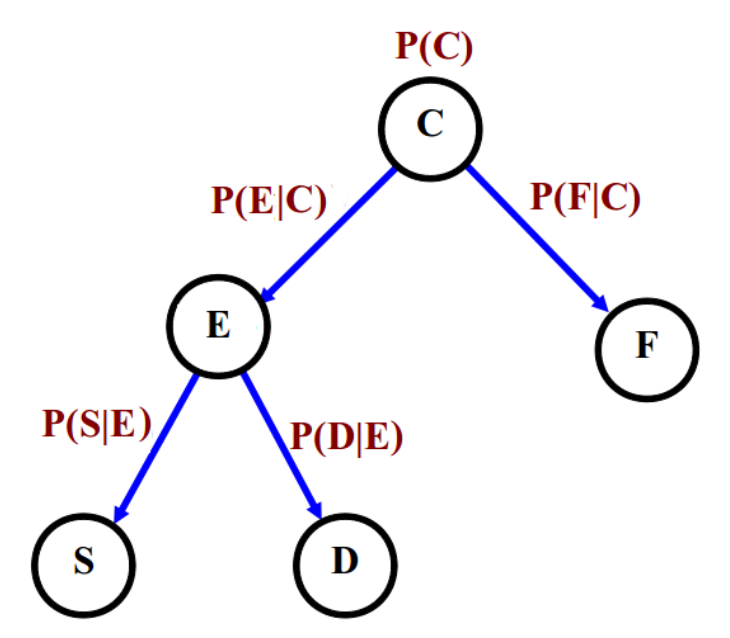
\includegraphics[width = 0.4\hsize]{./figures/NaiveBayes.png} % this includes the figure and specifies that it should span 0.7 times the horizontal size of the 
\caption{Example of naive bayes network. Given the parent $C$, the node $E$ and $F$ meet the causal markov condition, i.e. they are conditionally independent.} % caption of the figure
\label{fig:NaiveBayes} % a label. When we refer to this label from the text, the figure number is included automatically
\end{center}
\end{figure}

\item Each arc in a simple network is represented by a link matrix (conditional probability matrix)
\begin{align*}
\vec{P}(\vec{D}\vert \vec{C})&= \left[P(d_i \vert c_j) \right] = 
\begin{bmatrix}
P(d_1\vert c_1) & P(d_1\vert c_2) \\
P(d_2\vert c_1) & P(d_2\vert c_2) \\
P(d_3\vert c_1) & P(d_3\vert c_2) \\
P(d_4\vert c_1) & P(d_4\vert c_2) \\ 
\end{bmatrix}
\end{align*}

\item The root nodes of a network do not have any parents. They have a vector giving the prior probabilities
\begin{align*}
\vec{P}(\vec{C})&= \left[P(c_i) \right] = 
\begin{bmatrix}
P(c_1) & P(c_2) 
\end{bmatrix}
\end{align*}

\item \textbf{Instantiation} means setting the value of a node. 

\item \textbf{Bayesian Classifiers} using the above network. 

\begin{enumerate}
\item We cannot compute $E$ as it is a latent variable that we compute and we do not have measurements. However, we can computed the likelihood of $E$.
\begin{align*}
P(E \vert S\cap D) &= \alpha P(E)P(S\vert E)P(D\vert E)& = \alpha P(E) L(E\vert S \cap D)\\
L(E\vert S \cap D)& = (S\vert E)P(D\vert E)
\end{align*}  

\item Then we look at the root note $C$. Given $F=f_5$:
\begin{align*}
P(C \vert E \cap F)& = \alpha P(C) P(E\vert C)P(F\vert C)\\
P(e\vert c_k) &= \sum_{i=1}^3 P(e_i\vert c_k)L(e_i)\\
P^\prime (c_k)& = P(c_k\vert e \cap f_5)= \alpha P(c_k)\left(\sum_{i=1}^3 P(e_i\vert c_k)L(e_i)\right)P(f_5\vert c_k)
\end{align*}

\item We see the the evidence for C comes from
\begin{enumerate}
\item Evidence coming from $E$ and its sub-tree
\item Evidence from everywhere else.
\end{enumerate}
\begin{align*}
P_E(C) & = \alpha P(C) P(F\vert C)\\
\vec{P}(\vec{E}) & = \vec{P}(\vec{E}\vert \vec{C})\vec{P}_\vec{E}(\vec{C})
\end{align*}

\item Suppose if we have the instantiations $S=s_3$ and $D=d_2$
\begin{align*}
P^\prime(e_i) = \alpha P(e_i)P(s_3\vert e_i)P(d_2\vert e_i)
\end{align*}

\end{enumerate}

\end{enumerate}

\newpage

\section{Evidence and Message Passing: Pearl's Algorithm}

\begin{enumerate}
\item New concepts to deal with complex networks with intermediate nodes:
\begin{itemize}
\item \textbf{Evidence} is the information that we have at a node -this may be gathered through instantiation (exact value or virtual evidence), or inferred from passing messages. Evidence is unnormalized probabilities so the absolute values are meaningless, but they are useful for making comparisons.
\item \textbf{Messages} is the information (evidence) passed between nodes to provide evidence to another node.
\end{itemize}



\item \textbf{Theorem:} Let $(\mathbb{G}, P)$ be a Bayesian network whose DAG is a tree, where $\mathbb{G} = (V,E)$, and $a$ be a set of values of a subset $A\subset V$. 
\begin{enumerate}
\item \textbf{$\lambda$ messages}: For each child $Y$ of $X$, $\forall x \in X$
\begin{align*}
\lambda_Y(x) = \sum_y P(y\vert x)\lambda(y)
\end{align*}

\item \textbf{$\lambda$ values}: 
\begin{enumerate}
\item If $X\in A$ and $X$ is instantiated to $\hat{x}$
\begin{align*}
\lambda(\hat{x})& = 1,		\text{ for } x = \hat{x}&\\
\lambda(x) & = 0,				\text{ for } x\neq \hat{x}&
\end{align*}

\item if $X \notin A$ and $X$ is a leaf, $\forall x \in X$, 
\begin{align*}
\lambda(x) = 1
\end{align*}

\item If $X \notin A$ and $X$ is not a leaf, $\forall x \in X$
\begin{align*}
\lambda(x) = \prod_{U\in CH_X} \lambda_U (x),
\end{align*}
where $CH_X$ denotes the set of the children of $X$.
\end{enumerate}

\item  \textbf{$\pi$ messages}: If $Z$ is the parent of $X$, then $\forall z \in Z$
\begin{align*}
\pi_X(z) = \pi(z) \prod_{U\in CH_Z-\lbrace X\rbrace} \lambda_U(z)
\end{align*}

\item \textbf{$\pi$ values}:
\begin{enumerate}

\item If $X\in A$ and $X$ is instantiated to $\hat{x}$:
\begin{align*}
\pi(\hat{x})& = 1,		\text{ for } x = \hat{x}&\\
\pi(x) & = 0,				\text{ for } x\neq \hat{x}&
\end{align*}

\item If $X\notin A$ and $X$ is the root, $\forall x\in X $
\begin{align*}
\pi(X) = P(x)
\end{align*}

\item If $X\notin A$, X is not the root and $Z$ is the parent of $X$, $\forall x \ in X$
\begin{align*}
\pi(x) = \sum_z P(x\vert z) \pi_X(z)
\end{align*}

\end{enumerate}
\item Given the definitions, for each variable $X$, we have for all values of x,
\begin{align*}
P(x\vert a) = \alpha \lambda(x) \pi(x)
\end{align*}

\end{enumerate}

\item The $\pi$ values are basically evidence from the parents and it generalises the concept of prior. The $\lambda$ values are basically evidence from the descendents and it generalises the concept of likelihood probability.

\item Mnemonic: \textbf{p}i (\(\pi\)), \textbf{p}rior, and ``\textbf{p}arent'' all start with letter ``p''; and \textbf{l}ambda (\(\lambda\)), \textbf{l}ikelihood, and ``\textbf{l}ad'' all start with ``l''. Further, prior comes \textit{before} so from parents.

\item If we use virtual evidence at the leaf nodes, we can use the conditioning equation (above b(iii))

\begin{figure}[H]
\begin{center}
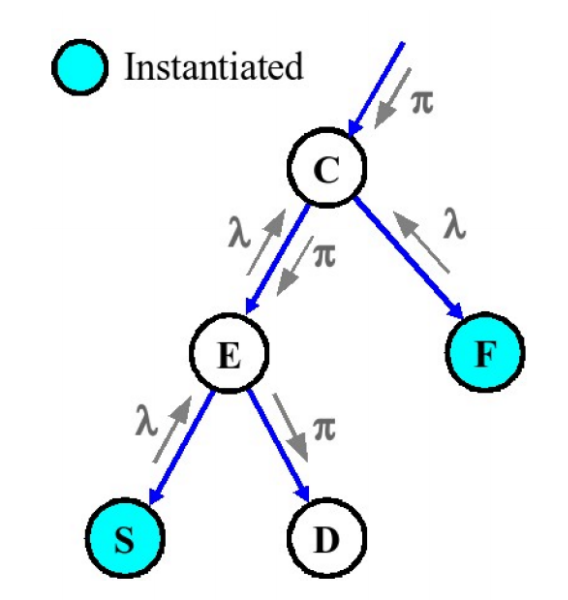
\includegraphics[width = 0.3\hsize]{./figures/PiLambda.png} % this includes the figure and specifies that it should span 0.7 times the horizontal size of the 
\caption{Upon instantiation of a node, we can propagate the $\lambda$ and $\pi$ messages} % caption of the figure
\label{fig:NaiveBayes} % a label. When we refer to this label from the text, the figure number is included automatically
\end{center}
\end{figure}

\item Important equations:
\begin{align*}
\vec{\lambda_S(E)}& = \vec{\lambda(S)P(S\vert E)} 		&	\vec{\pi(E)}& = \vec{P(E\vert C)\pi_E(C)}\\
\lambda(e_i) &= \prod_{CH_E} \left[\sum_{j} \lambda(s_j)P(s_j\vert e_i)\right] &
\pi(e_i)& = \sum_j \left[P(e_i\vert c_j)\pi(c_j)\prod_{k\backslash E}\lambda_k(c_j)\right]
\end{align*}

\item Notation
\begin{enumerate}
\item $\vec{\lambda_F(c)}$ means $\lambda$ evidence from node $F$ to node $C$.
\item $\vec{\pi_F(c)}$ means $\pi$ from all nodes besides $F$ for node $C$. (This can alternatively viewed as the information from $C$ to $F$)
\end{enumerate}


\end{enumerate}

\newpage

\section{Probability Propagation: Single Connected Networks}
\begin{enumerate}
\item A DAG is singly connected if there is at most one path between any two nodes. In a singly-connected network, each node can have more than 1 parents.
\item The main properties of these networks are:
\begin{enumerate}
\item The parents of a node are always independent given their common child (i.e. they don't have a common parent). This lets us calculate their joint probability as the product of their marginals.
\item When updating evidence of a node, the belief propagated through the net to update all nodes is guaranteed to reach a steady state.
\end{enumerate}

\item An example of a link matrix for a node with multiple parents looks as follows:
\begin{align*}
\mat{P(e|w,c)} = \begin{bmatrix} 
P(e_1|w_1,c_1) & P(e_1|w_1,c_2) & P(e_1|w_2,c_1) & P(e_1|w_2,c_2)\\ 
(e_2|w_1,c_1) & P(e_2|w_1,c_2) & P(e_2|w_2,c_1) & P(e_2|w_2,c_2) \\ 
P(e_3|w_1,c_1) & P(e_3|w_1,c_2) & P(e_3|w_2,c_1) & P(e_3|w_2,c_2) \end{bmatrix}
\end{align*}


\item To calculate the \(\pi\) evidence of a node with 2 parents (assuming independence between the parents): 
\begin{align*} 
\pi(\mat{E}) = \mat{P(e|w,c)}\mat{\pi_e(w,c)} = \mat{P(e|w,c)}\mat{\pi_e(w)\pi_e(c)}
\end{align*}

\item To calculate the \(\lambda\) evidence of a node with 2 parents, we have to calculate one \(\lambda\) message for each of the parents. If \(c\) has parents \(a\) and \(b\), then the evidence from \(c\) to \(a\) is as follows: 
\begin{align*} 
\lambda_c(a_i) = \sum_{j=1}^n\pi_{c}(b_j)\sum_{k=1}^m P(c_k|a_i,b)\lambda(c_k)
\end{align*}
where \(n\) is the number of values that \(b\) takes, and \(m\) is the number of values \(c\) takes. 


\item \textbf{Theorem:} Let $(\mathbb{G}, P)$ be a Bayesian network that is singly-connected, where $\mathbb{G} = (V,E)$, and $a$ be a set of values of a subset $A\subset V$. 
\begin{enumerate}
\item \textbf{$\lambda$ messages}: For each child $Y$ of $X$, $\forall x \in X$
\begin{align*}
\lambda_Y(x) = \sum_y \left[ \sum_{w_1,\dots, w_k} \left(P(y\vert x, w_i,\dots,w_k)\prod_{i=1}^k \pi_Y(w_i)\right)\right] \lambda(y)
\end{align*}
where $\lbrace W_i \rbrace_{i=1}^k$ are the other parents of $Y$.

\item \textbf{$\lambda$ values}: 
\begin{enumerate}
\item If $X\in A$ and $X$ is instantiated to $\hat{x}$
\begin{align*}
\lambda(\hat{x})& = 1,		\text{ for } x = \hat{x}&\\
\lambda(x) & = 0,				\text{ for } x\neq \hat{x}&
\end{align*}

\item if $X \notin A$ and $X$ is a leaf, $\forall x \in X$, 
\begin{align*}
\lambda(x) = 1
\end{align*}

\item If $X \notin A$ and $X$ is not a leaf, $\forall x \in X$
\begin{align*}
\lambda(x) = \prod_{U\in CH_X} \lambda_U (x),
\end{align*}
where $CH_X$ denotes the set of the children of $X$.
\end{enumerate}

\item  \textbf{$\pi$ messages}: If $Z$ is the parent of $X$, then $\forall z \in Z$
\begin{align*}
\pi_X(z) = \pi(z) \prod_{U\in CH_Z-\lbrace X\rbrace} \lambda_U(z)
\end{align*}

\item \textbf{$\pi$ values}:
\begin{enumerate}

\item If $X\in A$ and $X$ is instantiated to $\hat{x}$:
\begin{align*}
\pi(\hat{x})& = 1,		\text{ for } x = \hat{x}&\\
\pi(x) & = 0,				\text{ for } x\neq \hat{x}&
\end{align*}

\item If $X\notin A$ and $X$ is the root, $\forall x\in X $
\begin{align*}
\pi(X) = P(x)
\end{align*}

\item If $X\notin A$, X is not the root and $\lbrace Z_i \rbrace_{i=1}^j$ are the parents of $X$, $\forall x \ in X$
\begin{align*}
\pi(x) = \sum_{z_1,\dots, z_j} \left(P(x\vert z_1,\dots, z_j) \prod_{i=1}^j \pi_X(z_i)\right)
\end{align*}

\end{enumerate}
\item Given the definitions, for each variable $X$, we have for all values of x,
\begin{align*}
P(x\vert a) = \alpha \lambda(x) \pi(x)
\end{align*}

\end{enumerate}

\item \textbf{The Operating Equations for Probability Propagation}
\begin{enumerate}
\item {The $\lambda$ Message}
\begin{align*}
\lambda_C(a_i)& = \sum_{j=1}^m \pi_C(b_j) \sum_{k=1}^n P(c_k \vert a_i \cap b_j)\lambda(c_k)\\
&\\
\vec{\lambda_C(A)}&=\vec{\lambda(C)P(C\vert A)}\\
\lambda_C(a_i)& = \sum_{j=1}^m \pi_C(b_j) \lambda_C(a_i \cap b_j)
\end{align*}


\item {The $\pi$ Message:} If $C$ is a child of $A$, the $\pi$ message from $A$ to $C$ is:
\begin{align*}
\pi_C(a_i) & = \begin{cases}
1 													& \text{if $A$ is instantiated for $a_i$} \\
0 													& \text{if $A$ is instantiated but not for $a_i$} \\
P^\prime(a_i)/\lambda_C(a_i)		 	& \text{if $A$ is not instantiated}
\end{cases}
\end{align*}


\item {The $\lambda$ Evidence:} If $C$ is a node with $n$ children $D_1, \dots, D_n$, then the $\lambda$ evidence for $C$ is
\begin{align*}
\lambda(c_k) &=\begin{cases}
1											& \text{if $C$ is instantiated for $c_k$}\\
0											& \text{if $C$ is instantiated but not for $c_k$}\\
\prod_i \lambda_{D_i}(c_k)	& \text{if $C$ is not instantiated}
\end{cases}
\end{align*}

\item {The $\pi$ Evidence:} If $C$ is a child of two parents $A$ and $B$, the $pi$ evidence for $C$ is:
\begin{align*}
\pi(c_k)& = \sum_{i=1}^l \sum_{j=1}^m P(c_k \vert a_i \cap b_j)\pi_C(a_i)\pi_C(b_i)\\
\vec{\pi(C)}& = \vec{P(C\vert A)\pi_C(A)}
\end{align*}

\item {The Posterior Probabilities:} If $C$ is a variable, the posterior probability of $C$ based on the evidence received is
\begin{align*}
P^\prime(c_k) = \alpha \lambda(c_k) \pi(c_k)
\end{align*}
\end{enumerate}

\begin{figure}[H]
\begin{center}
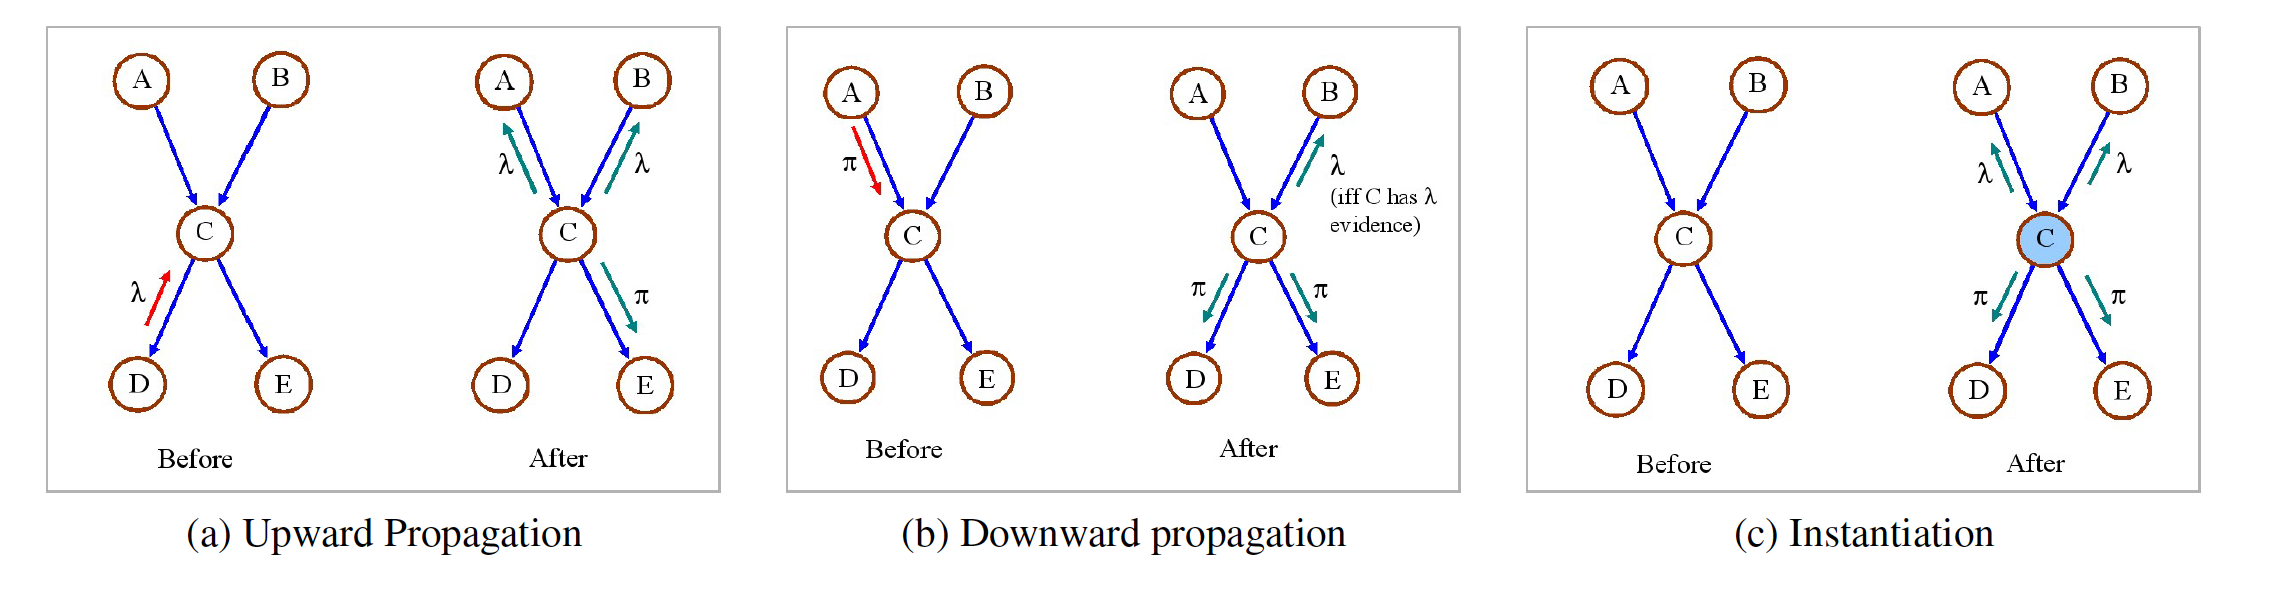
\includegraphics[width = 1.00\hsize]{./figures/ProbabilityPropagation.png} % this includes the figure and specifies that it should span 0.7 times the horizontal size of the 
\caption{Probability propagation} % caption of the figure
\label{fig:NaiveBayes} % a label. When we refer to this label from the text, the figure number is included automatically
\end{center}
\end{figure}

\item \textbf{Message Passing}
\begin{enumerate}
\item \textbf{Initialization:} For all the root nodes, the $\pi$ values are set to the prior probabilities and propagate the $\pi$ messages using downward propagation
\item \textbf{Upward Propagation (only for uninstantiated nodes):} A node $C$ receives $\lambda$ from a child. 
\begin{itemize}
\item Compute the new $\lambda(C)$ and $P^\prime(C)$. Then, post a $\lambda$ message to all its parents and post a $\pi$ message to all $C$'s other children.
\end{itemize}
\item \textbf{Downward Propagation:} If a variable $C$ receives a $\pi$ message from one parent.
\begin{itemize}
\item If $C$ is not instantiated: Compute $\pi(C)$ and $P^\prime(C)$ and post $\pi$ message to each child.
\item If there is evidence in $C$: Post $\lambda$ message to the other parents
\end{itemize}

\item \textbf{Instantiation:} If $C$ is instantiated for state $c_k$,
\begin{itemize}
\item $P^\prime (c_k) =1$ and $P^\prime (c_j) = 0 \forall j\neq k$. Compute $\lambda (C)$
\item Post $\lambda$ and $\pi$ message to each parent and each child of $C$ respectively.
\end{itemize}
\end{enumerate}

\begin{figure}[H]
\begin{center}
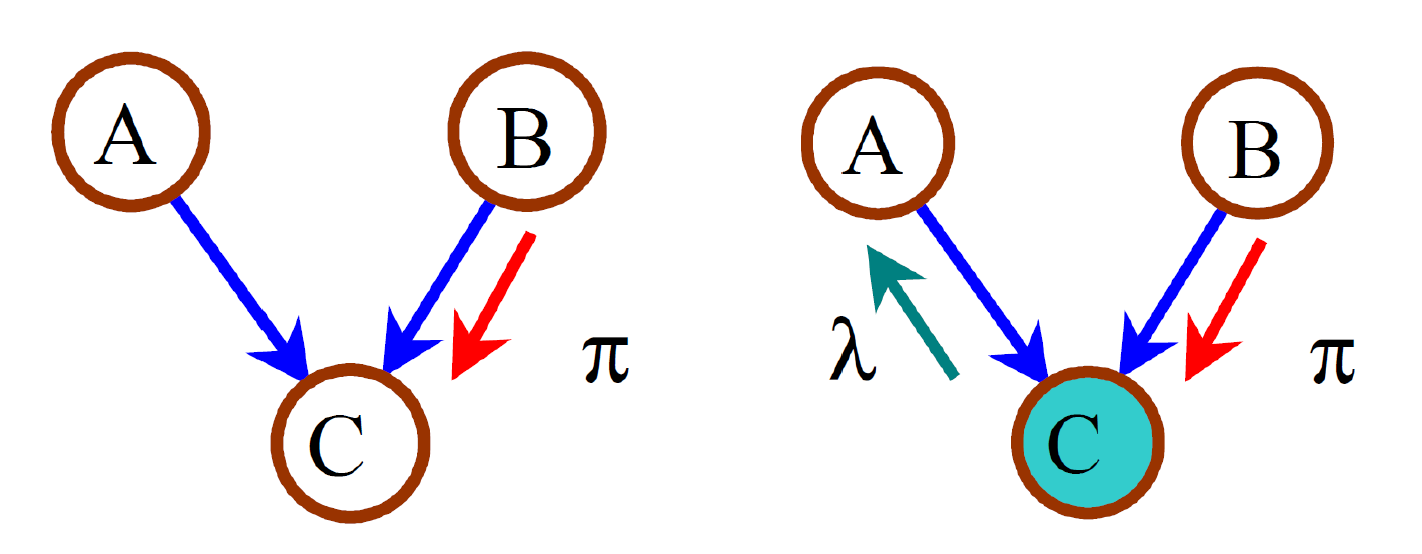
\includegraphics[width = 0.50\hsize]{./figures/ConvergingConnection.png} % this includes the figure and specifies that it should span 0.7 times the horizontal size of the 
\caption{Converging Connections} % caption of the figure
\label{fig:NaiveBayes} % a label. When we refer to this label from the text, the figure number is included automatically
\end{center}
\end{figure}

\begin{figure}[H]
\begin{center}
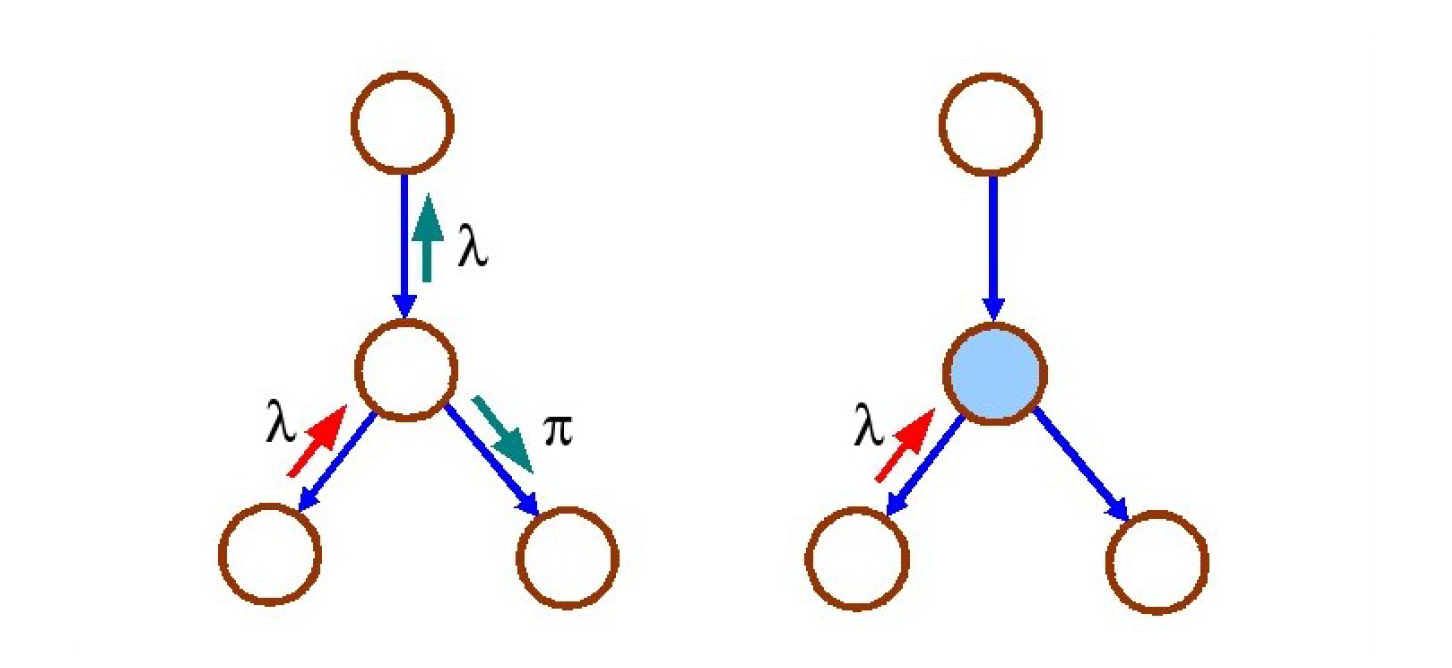
\includegraphics[width = 0.55\hsize]{./figures/DivergingConnection.png} % this includes the figure and specifies that it should span 0.7 times the horizontal size of the 
\caption{Diverging Connection} % caption of the figure
\label{fig:NaiveBayes} % a label. When we refer to this label from the text, the figure number is included automatically
\end{center}
\end{figure}


\item \textbf{Blocked Path (very important to understand this):}
\begin{itemize}
\item For a diverging path: when the node is instantiated, it will block the passing message between other nodes.
\item For a converging path: it is blocked when there is no $\lambda$ evidence on the child node, but unblocked when there is $\lambda$ evidence or when the node is instantiated.

\begin{align*}
\lambda_C(a_i)& = \sum_{j=1}^m \pi_C (b_j) \sum_{k=1}^n P(c_k \vert a_i \cap b_j) \lambda(c_k)\\
\lambda(c_k) & = 1, \forall c_k \Rightarrow \lambda_C(a_i) = \sum_{j=1}^m \pi_C (b_j) 
\end{align*}
\end{itemize}

\end{enumerate}

\newpage

\section{Building Networks from Data}

\begin{enumerate}
\item Building networks from data:
\begin{enumerate}
\item \textbf{Expert knowledge}: We can obtained the network structure would be known or readily obtainable from an expert. This approach is highly subjective and reliant on the expert advice.
\item \textbf{Spanning tree algorithms}: Main idea is to start with a set of nodes to which we add arcs until a complete network is created.
\begin{enumerate}
\item The nodes that are joined by arcs are depedent and those not are at least conditionally independent. Hence the strategy is to add arcs that connect variables that are most dependent.
\item For every pair of variables calculate the dependency. Then join the nodes in dependency order, provided the resulting structure has no loops
\end{enumerate}
\end{enumerate}

\item \textbf{Adding Causal Directions:}
\begin{enumerate}
\item If a node is considered a root node, we will point all arrows from it. 
\item On the whole, cause is a semantic entity that needs human intervention to determine.
\end{enumerate}


\item \textbf{Measures of dependencies}
\begin{itemize}
\item \textbf{$L1$ dependency measure}:
\begin{align*}
Dep (A,B) & = \sum_{A\times B} \left\vert P(a_i \cap b_j) - P(a_i)P(b_j)\right\vert \\
Dep (A,B) & = \sum_{A\times B} P(a_i \cap b_j) \times \left\vert P(a_i \cap b_j) - P(a_i)P(b_j)\right\vert 
\end{align*}
\item \textbf{$L2$ dependency measure}:
\begin{align*}
Dep (A,B) & = \sum_{A\times B} \left(P(a_i \cap b_j) - P(a_i)P(b_j)\right)^2\\
Dep (A,B) & = \sum_{A\times B} P(a_i \cap b_j) \times \left(P(a_i \cap b_j) - P(a_i)P(b_j)\right)^2
\end{align*}
As the probabilities becomes small they contribute less to the dependency, and this effect is acceptable since we have little information on rare events. 
The weighted version of the $L1$ and $L2$ further reduces the dependency for low probability values.

\item \textbf{Kullback-Leibler Measure (mutual entropy)}
\begin{itemize}
\item It is zero when two variables are completely independent
\item It is positive and increasing with dependency when applied to probability distributions
\item It is independent of the actual value of probability
\item Can be computed as follows
\begin{align*}
Dep(A,B)& = \sum_{A\times B} P(a_i \cap b_j) \log_2\left[\frac{P(a_i \cap b_j)}{P(a_i)P(b_j)}\right]
\end{align*}

\end{itemize}

\item \textbf{Correlation}
\begin{itemize}
\item Measures only linear dependency whereas mutual entropy can characterise higher order dependencies more accurately.
\item Can be computed as follows:
\begin{align*}
C(A,B) & = \frac{\Sigma_{AB}}{\sqrt{\sigma_A\sigma_B}}\\
\Sigma_{AB}& = \frac{1}{N-1}\sum_{i=1}^N (a_i -\bar{a}_i)(b_i -\bar{b}_i)\\
\sigma_A& = \frac{1}{N-1}\sum_{i=1}^N (a_i -\bar{a}_i)^2
\end{align*}
\end{itemize}
\end{itemize}

\end{enumerate}







\section{Cause and Independence}



\begin{enumerate}
\item Independence: In a network, if there is no path between two variables, they are independent. 
\begin{itemize}
\item Two variables can be connected by a path in a network and still be independent as the conditional probability can express no dependency.
\item In theory, the absence of an arc is more significant than the presence of an arc. However, in theory we avoid arcs with very low dependency in networks.
\item The spanning tree algorithm can be terminated when the dependecy becomes too low to be significant.
\end{itemize}

\item (d-separation) Let $\mathbb{G}=(V,E)$ be a DAG, $A\subseteq V$ and $X$ and $Y$ be distinct nodes in $V-A$. $X$ and $Y$ are d-separated by $A$ in $\mathbb{G}$ if every chain between $X$ and $Y$ is blocked by $A$.

\item Possible configurations of connected triplets:
\begin{figure}[H]
\begin{center}
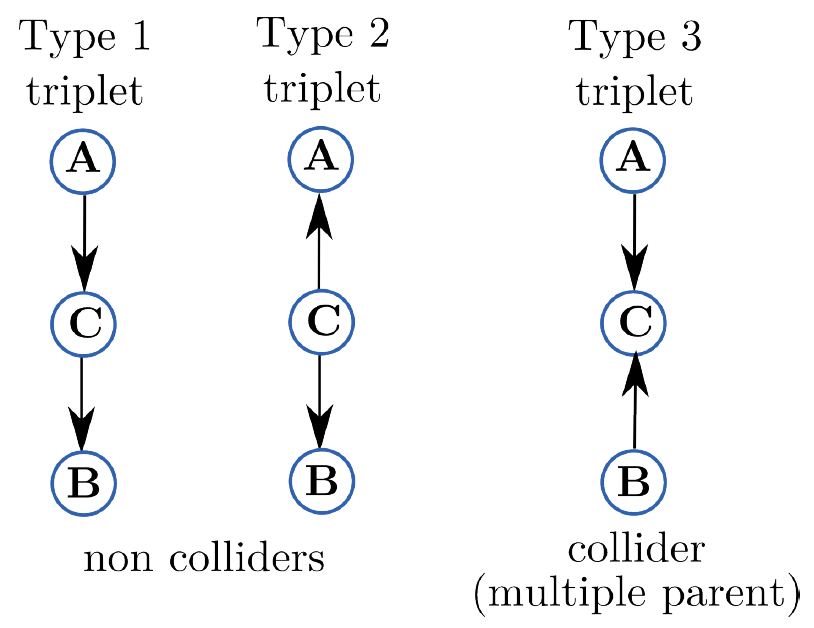
\includegraphics[width = 0.4\hsize]{./figures/TripletConfig.png} % this includes the figure and specifies that it should span 0.7 times the horizontal size of the 
\caption{Possible configurations of connected triplets.} % caption of the figure
\label{fig:NaiveBayes} % a label. When we refer to this label from the text, the figure number is included automatically
\end{center}
\end{figure}

\begin{enumerate}
\item \textbf{Non-colliders}: If $C$ is instantiated, no messages pass from $A$ to $B$.
\item \textbf{Colliders:} The nodes $A$ and $B$ are independent if there is no information on C. 
	\begin{itemize}
		\item Marginal Independence: We can measure the dependence between A and B using all the data. If this is low, the configuration may be multiple parent.
		\item Conditional Independence: We can partition data according to states of C and compute the dependency between A and B. If this is high, the configuration may be multiple parent.
		\begin{figure}[H]
			\begin{center}
				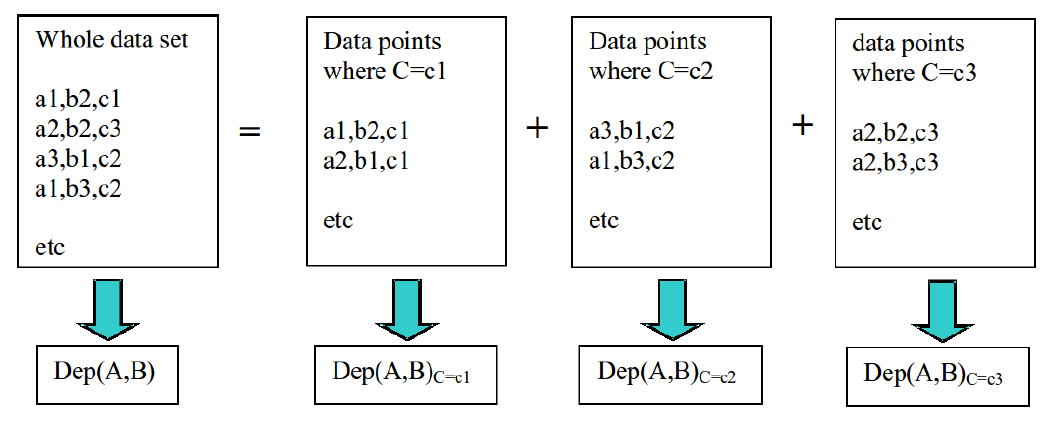
\includegraphics[width = 0.8\hsize]{./figures/MultParent.png} % this includes the figure and specifies that it should span 0.7 times the horizontal size of the 
				\caption{Practical computation.} % caption of the figure
				\label{fig:NaiveBayes} % a label. When we refer to this label from the text, the figure number is included automatically
			\end{center}
		\end{figure}			
	\end{itemize}
\end{enumerate}

\item  \textbf{Determining Causal Directions:} 
	\begin{enumerate}
		\item Compute the maximally weighted spanning tree
		\item For each connected triplet in the spanning tree
		\begin{itemize}
			\item Compute the joint probability of the triplet
			\item Compute the marginal dependence and condition dependence
			\item If marginal dependence is low and the conditional dependence is high, put in causal directions corresponding to a collider			
		\end{itemize}
		\item Propagate the causal arrows as far as possible
	\end{enumerate}

\item Structure and Parameter Learning
	\begin{itemize}
		\item Bayesian networks 
			\begin{itemize}
				\item Combined both structure and parameter learning. 
				\item We can express our knowledge by choosing the structure or we can learn it through data.
				\item Incorporate known causal relations but have the potential to learn cause from data.
			\end{itemize}
		\item Neural networks
			\begin{itemize}		
		 		\item Offers only parameter learning. 
		 		\item It is difficult to embed knowledge or infer structure from a neural network.
		 		\item Most applicable when we have no causal knowledge but we cannot extract causal information from them.
		 	\end{itemize}
		\item Rule based system (logic based)
			\begin{itemize}
				\item Have just structure but they are not scalable and difficult to optimise.
				\item Most applicable when we have causal knowledge as these systems can represent it well
			\end{itemize}
	\end{itemize}


\end{enumerate}




\section{Model Accuracy}
\begin{enumerate}
    \item The model may be evaluated using  \textbf{maximum likelihood estimation}.
		\begin{align*}
			P(Ds|Bn) 	&= \prod_{data} P(Bn)\\
							&= \prod_{i} P(x_i)P(y_i\vert x_i) \text{ (case of two variables)}
		\end{align*}		    
    
        \begin{itemize}
            \item Above is the general formulation, but to avoid underflow errors, one may take the log likelihood. If the log we take is base 2, then the log likelihood is known as the information measure since 
            			$\log_2$ N bits are required to represent integers up to $N$.
				\begin{align*}
					\log(P(Ds|Bn)) = \sum_{data} log(P(Bn))
				\end{align*}            

            \item $Ds$ is a given dataset, $Bn$ is a our BayesNet model, and $\prod_{data}P(Bn)$ is the joint probability of the model multiplied over all values in the dataset.
            \item Larger models get higher scores, so size becomes a confounding variable.
        \end{itemize}
        
    \item \textbf{Minimum Description Length Score} (MDLScore, also known as Bayesian Information Criterion) penalises larger models to provide a fair comparison for smaller models. The size of the model is characterized by the number of parameters.
			\begin{align*}
				MDLScore = \frac{\vert B_n \vert}{2}\log_2 N -\log_2 P(D_s\vert B_n)
			\end{align*}			    
    
        \begin{itemize}
        	\item A gentle reminder of principle of parsimony or Occam's Razor: A simple model is preferred to a complex model. 
        	\item The first part of the above equation is the average number of bits required to store the values. 
            \item \textbf{Example}. If a network has a parent and a child, and we have 4 datapoints ($N=4$, each node takes 2 values), the parent has a prior probability of 2 parameters, and the conditional table has $2\times2 =4 $. Therefore, $Size(Bn|Ds) = |Bn|log_2(4)/2 = [(2-1) + (2-1)\times2]log_2(4)/2  = 3 \times 2/2 = 3$.
            \item MDL Score is not an absolute measure. It can only be used to compare two models of the same data set.
            \item \textbf{need to add why this is a better measure than euclidean distance (from tutorial)}
        \end{itemize}
               
        
	\item \textbf{Measuring Predictive Accuracy}: Split the data into training data and test data, then use the test data to measure the network accuracy. It can be used to minimize the number of variables in a spanning tree.
		\begin{itemize}
			\item Build a spanning tree and obtain an ordering of the nodes starting at the root.
			\item Remove all the arcs.
			\item Add arcs in the order of their dependency.
			\item If the predictive accuracy is good enough, stop. Else, go back to 3rd step.
		\end{itemize}			
	
\end{enumerate}

\section{Approximate Inference}
\begin{enumerate}

	\item For highly dependent data, we can:
		\begin{enumerate}
			\item Model all dependencies - Propagation of probabilities is difficult or infeasible.
			\item Maximally weighted spanning tree - Does not model dependencies accurately but message passing terminates in one pass and it is very fast.
		\end{enumerate}
		
	\item Problems with loops in networks:
		\begin{enumerate}
			\item Looping messages.
			\item Independence of multiple parents.
		\end{enumerate}	
	
	\item Approximate Inference Methods:
		\begin{itemize}
			\item Node deletion (Seletive Bayes Network)
			\item Loopy belief propagation
			\item Hidden / latent node placement
		\end{itemize}
		
	\item \textbf{Node Deletion and Selective Bayes Network}: Main idea is to use a subset of the variables.
		\begin{itemize}
			\item Start with a network with all variables then deleting any variables and testing the improvement.
			\item Alternatively, add variables incrementally and test the performance for each network.
		\end{itemize}
		
	\item \textbf{Loopy Belief Propagation}: Include all arcs expressing significant dependency and allow propagation to continue until
		\begin{itemize}
			\item The probability distributions reach a stable state; or
			\item A limiting number of iterations has occurrec (i.e. there may be no steady state)
		\end{itemize}

	\item \textbf{Hidden Nodes}: If any two children of a parent are not conditionally independent, they can be separated by hidden node.
		\begin{itemize}
			\item Switch nodes: Hidden nodes can act as switches to simplify the networks.
			\item A network can always perform as well with a hidden node as it can without.
		\end{itemize}
			
\end{enumerate}



\subsection{Using Hidden Nodes}

\begin{enumerate}
\item To create a hidden note, we need to decide:
	\begin{itemize}
		\item How many states it should have.
		\item Identify values for the 3 new linked matrices introduced.
	\end{itemize}

\item Determination of number of states:
	\begin{itemize}
		\item Number of states for hidden node will be comparable to the number of states of the nodes it is separating.
		\item Expect the hidden node to have at least the same number of states of its parent.
		\item Linked matrices with too many states will have low probabilities for some states. Hence, start with large number of states and then reduce them.
	\end{itemize}

\item Calculating the linked matrices (conditional probabilities)
	\begin{enumerate}
		\item Given the estimates of $P(H\vert A)$, $P(B\vert H)$, $P(C\vert H)$ and a set of data points $[a_i, b_j, c_k]$.
		\item Use each $b_j$, $c_k$ to compute $P^\prime (A)$ from the network, calculate and accumulate the error
			\begin{align*}
				E = [P^\prime (A) - P(a_i)]^2
			\end{align*}
		\item Minimize $E$ over the data set by adjusted $P(H\vert A)$, $P(B\vert H)$, $P(C\vert H)$ using the gradient descent algorithm
			\begin{align*}
				P(h_k \vert a_j) &\rightarrow P(h_k \vert a_j)- \mu \frac{\partial E}{\partial P(h_k \vert a_j)}\\
				P(b_j \vert h_k) &\rightarrow P(b_j \vert h_k) - \mu \frac{\partial E}{\partial P(b_j \vert h_k)}\\
				P(c_j \vert h_k) &\rightarrow P(c_j \vert h_k) - \mu \frac{\partial E}{\partial P(c_j \vert h_k)}
			\end{align*}
		\item Using gradient descent may not actually arrive at the optimal answer due to the following issues:
			\begin{itemize}
				\item Distributions will no longer sum to 1.
				\item Individual probability values may be greater than 1 or less than 0.
				\item Conditional probability matrices need to be normalized and this may compromise finding an optimum solution.
			\end{itemize}					
		
	\end{enumerate}




\end{enumerate}







\section{Exact Inference}

\section{Probability Propagation: Join Trees}



\end{document}
%%% Local Variables: 
%%% mode: latex
%%% TeX-master: t
%%% End: 
